\section{Methods}

To archive clustering, the method adopted was to compare document using the authorship linkings presented in \cite{kocher_verification}.
In this study was to compare the following possible text representation to compare document based on author style : words frequencies, lemma frequencies, Part-Of-Speach (POS) tags frequencies, as well as n-grams frequencies.
The distance mesures used are : $L^1$ norms (Manhattan, Tanimoto), $L^2$ norm (Matusita, Clark), inner products (Cosine distance) and the Jeffery divergence.
Depending on the dataset, the text representation and the metric used, different distance mesures were giving better results.

In this study to archive a good clustering, the main objective is to have a reliable authorship linking rank list.
To try to increase the quality of the rank list, the proposed method is to use a combination of multiple rank list using to form a new rank list.

\subsection{Authorship linking}

\subsubsection{Rank list fusion}

Each rank list is ordered using a different distance measure.
The order of magnitude of each rank list is different.
To avoid this problem, the solution opted is to only use the rank of each link.

An additional constraint desired is to favor top ranked link and penalize bottom ranked links when fusing rank lists.
This constraint can be easily explained by observing the distance over the rank graph of the rank list.
Figure~\ref{fig:distance_over_rank} clearly show us the top ranked links and bottom ranked links are fewer than the middle section.

\begin{figure}
  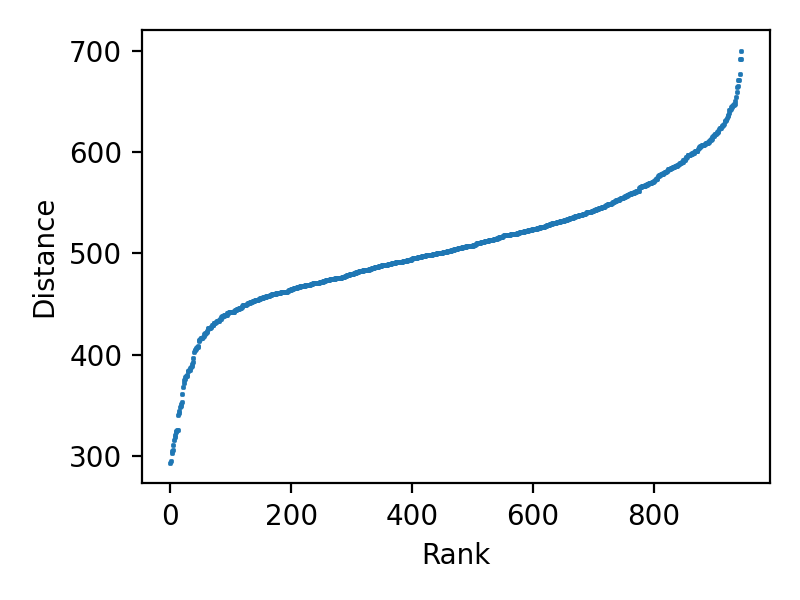
\includegraphics[width=\linewidth]{img/distance_over_rank.png}
  \caption{Distance over rank in the links of the Brunet dataset using Manhattan distances using the 500 most frequent tokens.}
  \label{fig:distance_over_rank}
\end{figure}

Which correspond to correctly correlated documents (top links) and negatively correlated documents (bottom links).
Assuming that the top rank are true links after the rank list fusion these link should also be top rank.
The same reasoning can be apply for the bottom links.

Using the reciprocal of the sigmoid function we can modelize such curve. Sigmoid functions presented in Equation~\ref{eq:sigmoid} and Figure~\ref{fig:sigmoid}. It's reciprocal in Equation~\ref{eq:sigmoid_r} and Figure~\ref{fig:sigmoid_reciprocal}

\begin{equation}
  \label{eq:sigmoid}
  S(x) = \frac{1}{1+e^-x}
\end{equation}
\begin{equation}
  \label{eq:sigmoid_r}
  S^{-1}(x) = -\ln{\frac{x-1}{x}}
\end{equation}

\begin{figure}
  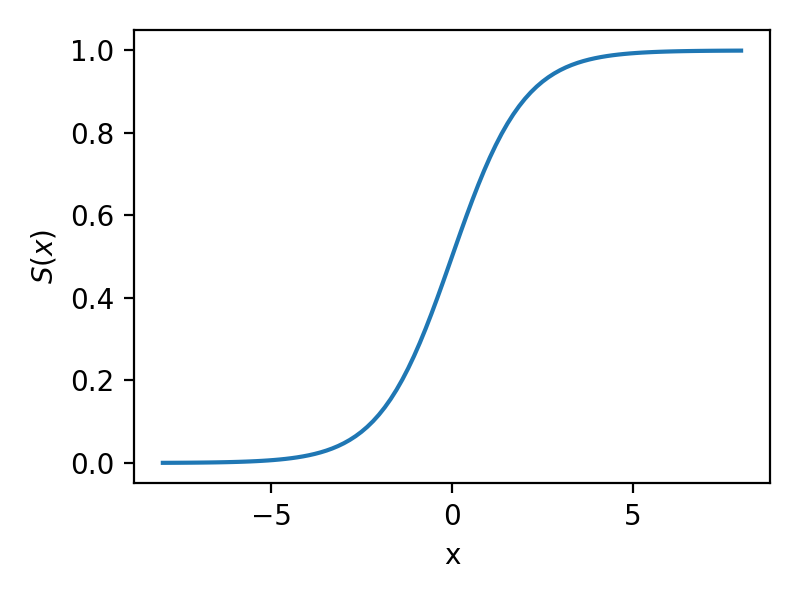
\includegraphics[width=\linewidth]{img/sigmoid.png}
  \caption{Sigmoid function between -8 and 8}
  \label{fig:sigmoid}
\end{figure}
\begin{figure}
  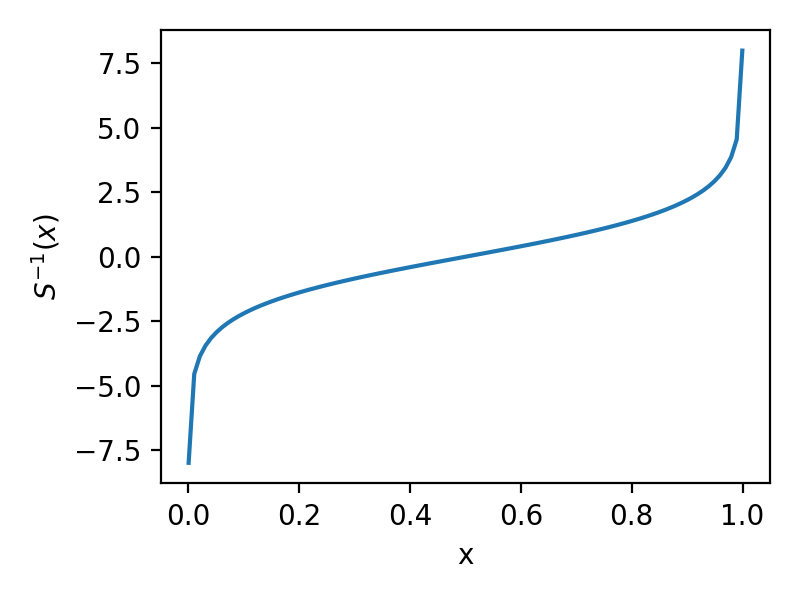
\includegraphics[width=\linewidth]{img/sigmoid_reciprocal.png}
  \caption{Reciprocal of the sigmoid function between sigmoid(-8) and sigmoid(8)}
  \label{fig:sigmoid_reciprocal}
\end{figure}

\subsection{Authors Clustering}

To find clusters of authors, a possible way is to use aglomeratives clustering on a rank list.
